\chapter{TINJAUAN PUSTAKA}
\label{chap:tinjauanpustaka}

Demi mendukung implementasi pada tugas akhir, penelitian atau perancangan terdahulu dan dasar teori
yang berkaitan akan dijelaskan pada bab ini. Hasil kajian yang didapat
dan dasar teori tersebut akan digunakan pada tugas akhir.

\section{Penelitian atau Perancangan Terdahulu}

\subsection{ViteraaS: Virtual Cluster as a Service}

Paper ini mengangkat studi kasus mengenai penggunaan sumber daya komputasi
yang dimiliki oleh sebuah universitas. Sumber daya komputasi yang dimiliki
oleh universitas tersebut seperti PC dan server tidak termanfaatkan dengan
baik seperti saat malam hari karena tidak banyak mahasiswa yang menggunakannya.
Namun, sumber daya komputasi tersebut akan sangat padat penggunaannya saat
mendekati akhir semester dengan banyaknya tugas yang diberikan.

Dengan studi kasus tersebut, penulis dari penelitian ini mengajukan sebuah
platform bernama ViteraaS (Virtual Cluster as a Service). Platform tersebut
digunakan untuk membuat \emph{virtual cluster} dari \emph{pool} sumber daya
komputasi yang dimiliki oleh universitas. ViteraaS terintegrasi dengan
infrastruktur universitas seperti \emph{Single Sign-On} (SSO). Untuk mengatur
infrastruktur virtual seperti membuat klaster \emph{virtual machine} secara dinamik,
ViteraaS menggunakan OpenNebula \parencite{6133210}.

\section{Dasar Teori}

\subsection{Kubernetes}
\label{sec:kubernetes}

Kubernetes adalah sebuah platform manajemen aplikasi yang dikemas (\emph{containerized applications})
bersifat sumber terbuka. Kubernetes dibuat berdasarkan \emph{tool} internal yang
diciptakan oleh Google bernama Borg untuk mengelola layanan mereka dalam bentuk \emph{container},
kemudian beberapa pengembang Borg menciptakan platform serupa
namun bersifat sumber terbuka yang diberi nama Kubernetes \parencite{borg-references}.

Kubernetes dapat mengelola jalannya aplikasi berbasis kontainer seperti membuat
aplikasi tersebut \emph{scalable} dengan cara menambah atau mengurangi \emph{container}
yang menjalankan aplikasi tersebut sesuai dengan kebutuhan pengguna. Untuk memenuhi
hal tersebut, Kubernetes menyediakan beberapa fitur seperti berikut:

\begin{enumerate}

  \item \emph{Service discovery} dan \emph{load balancing}

    \emph{Container} pada Kubernetes diekspos oleh Kubernetes menggunakan DNS atau IP dari
    \emph{container} tersebut. Jika \emph{traffic} menuju \emph{container} tersebut tinggi, Kubernetes
    dapat menggunakan \emph{load balancer} sehingga \emph{traffic} dialihkan ke \emph{container} lain yang sejenis
    agar \emph{deployment} tetap stabil. Selain itu, dengan \emph{load balancing}, \emph{request} dapat ditangani
    dengan cepat tanpa perlu menunggu \emph{container} memroses semua \emph{traffic}
    yang tinggi.

  \item{Orkestrasi penyimpanan}

    Kubernetes dapat menggunakan beberapa jenis sistem penyimpanan, seperti
    penyimpanan lokal, penyimpanan dari penyedia jasa \emph{cloud}, dan sebagainya.
    Penyimpanan ini akan digunakan untuk banyak skenario, seperti penyediaan penyimpanan
    sementara untuk Pod, membagi sebuah \emph{filesystem} antara dua \emph{container}
    yang berbeda dalam satu Pod, membagi sebuah \emph{filesystem} antara dua Pod yang
    berbeda, dan lain-lain.

  \item \emph{Rollouts} dan \emph{rollbacks} secara otomatis

    Kubernetes dapat menyesuaikan \emph{state} dari konfigurasi \emph{state} yang
    diberikan, sehingga status dari \emph{state} klaster Kubernetes akan selalu mengikuti
    \emph{state} yang diberikan. \emph{Rollouts} pada Kubernetes menghasilkan versi terbaru
    dari sebuah aplikasi pada sebuah klaster. Proses \emph{rollouts} berjalan secara inkremental.
    \emph{Rollbacks} adalah sebuah proses untuk kembali ke versi atau \emph{state} sebelumnya apabila
    \emph{state} yang baru mengalami masalah atau tidak stabil.
    

  \item \emph{Self-healing}

    Kubernetes memiliki fitur \emph{self-healing} sehingga Kubernetes
    akan memulai ulang \emph{container} yang gagal atau mati dalam
    mengerjakan \emph{job}, menggantikan \emph{container}, dan akan selalu menunggu
    \emph{container} yang belum siap sebelum pengguna dapat menggunakannya. Dengan begitu,
    semua komponen pada klaster Kubernetes harus berada pada posisi yang sudah siap
    sebelum dapat digunakan.

    
  \item \emph{Horizontal scaling}

    Aplikasi yang di-\emph{deploy} pada Kubernetes dapat di-\emph{scaling} secara
    \emph{horizontal}, yaitu penambahan Pod untuk pengerjaan aplikasi tersebut. Proses
    ini terjadi secara otomatis jika \emph{workload} yang diterima oleh klaster lebih tinggi
    dari kemampuan klaster dalam menangani \emph{workload} tersebut. Jika \emph{workload}
    sudah mulai berkurang dan jumlah Pod di atas dari konfigurasi jumlah minimum Pod, maka
    tambahan Pod yang dibuat untuk menangani \emph{workload} yang tinggi tersebut akan dikurangi.
    
  \item IPv4 dan IPv6 \emph{dual-stack}

    Kubernetes dapat menggunakan IPv4 dan/atau IPv6 untuk alamat IP dari objek dalam Kubernetes.
    Penggunaan alamat IP untuk objek pada klaster Kubernetes dapat berupa ipv4 saja, ipv6 saja, atau
    penggunaan keduanya.
    
  \item Desain untuk ekstensibilitas

    Kubernetes didesain agar mudah dieksten tanpa merubah \emph{source code} dari Kubernetes.
    Salah satu contoh dari ekstensi yang bisa dilakukan tanpa merubah \emph{source code}
    dari Kubernetes adalah \emph{Custom Resources}. Pengguna klaster Kubernetes dapat
    membuat sebuah \emph{resource} baru menggunakan \emph{Custom Resources} tersebut. \emph{Resource}
    tersebut dapat berupa API khusus.

    \clearpage
    
\end{enumerate}

\subsubsection{Arsitektur Kubernetes}

Kubernetes menggunakan konsep klaster yang merupakan kumpulan dari satu atau
lebih server. Klaster Kubernetes terdiri dari satu buah server atau satu kelompok server yang
bertugas menjadi \emph{control plane} dan server lainnya menjadi \emph{worker node}.
Server atau kelompok server \emph{control plane} bertugas untuk mengatur jalannya
server lain yang menjadi \emph{worker node}, seperti melakukan \emph{health checking} serta
\emph{scheduling} pada \emph{worker node}, sedangkan server yang menjadi \emph{worker node}
bertugas untuk menerima dan melakukan pekerjaan yang diberikan oleh \emph{control plane}
dengan menggunakan sumber daya yang ada pada klaster. Arsitektur
klaster Kubernetes dapat dilihat pada gambar \ref{fig:arsitektur-cluster-kubernetes}

\begin{figure}[H]
  \centering
  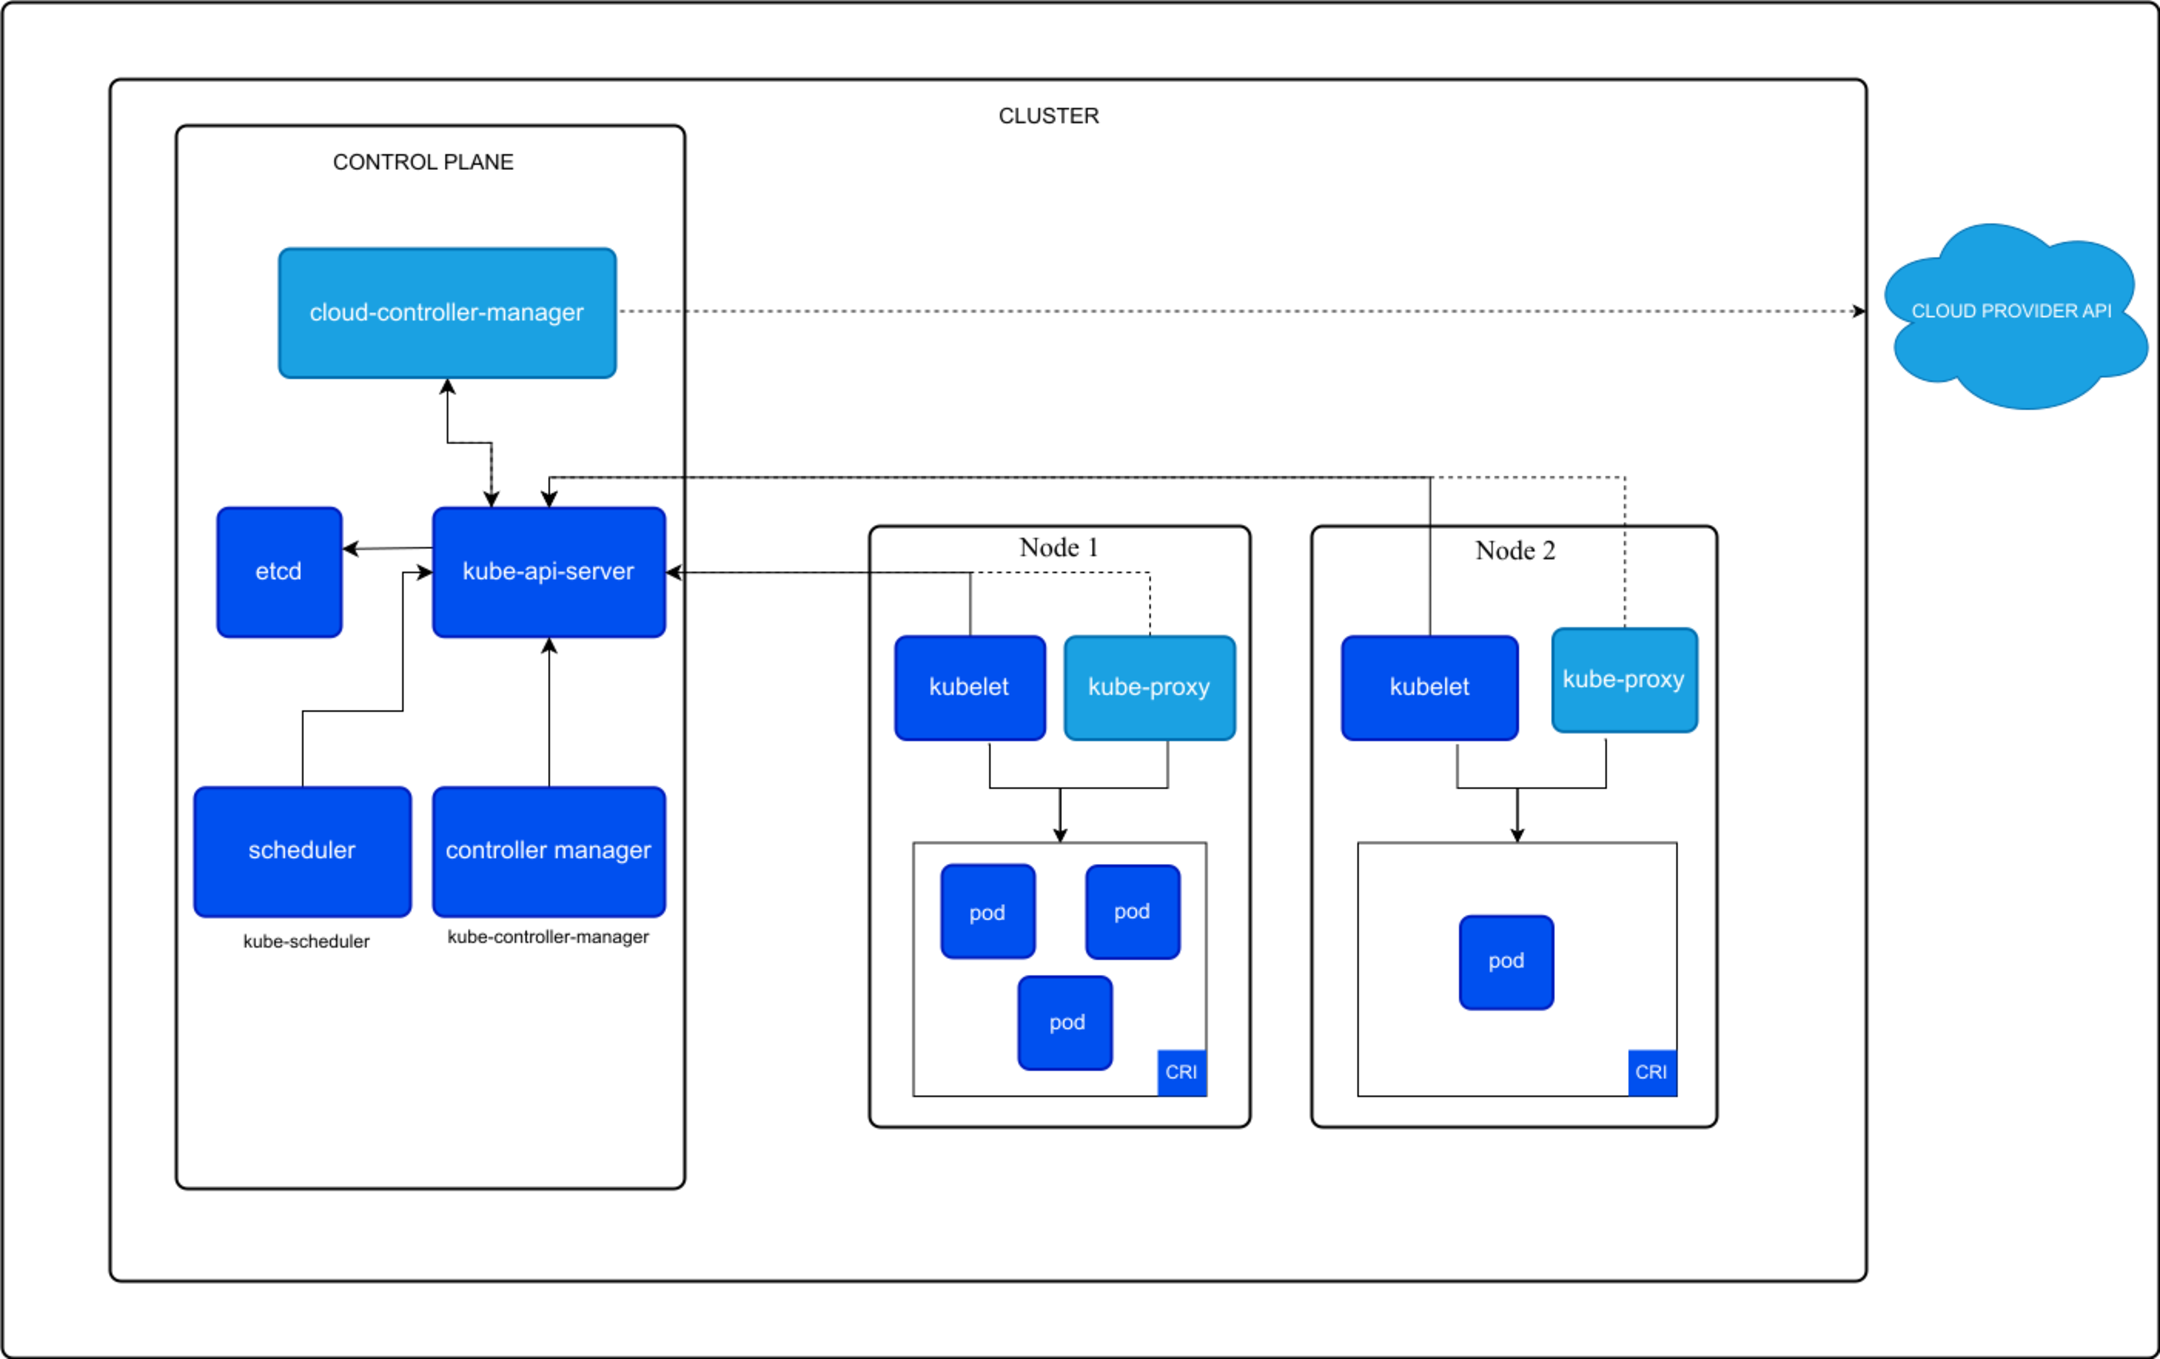
\includegraphics[scale=0.15]{gambar/kubernetes-cluster-architecture.png}
  \caption{Arsitektur Klaster Kubernetes}
  \label{fig:arsitektur-cluster-kubernetes}
\end{figure}

Dalam proses pembuatan klaster Kubernetes, Kubernetes menyediakan \emph{binary} pembantu
yang memudahkan pembuatan bernama kubeadm. Untuk membuat sebuah klaster Kubernetes,
server yang digunakan sebagai \emph{control plane} harus terlebih dahulu menginisiasi
pembuatan klaster. Setelah server \emph{control plane} telah selesai dalam menginisiasi klaster,
server yang digunakan sebagai \emph{worker node} akan digabungkan ke dalam klaster yang sebelumnya
telah dibuat oleh \emph{control plane}. Untuk memudahkan dalam pembuatan klaster, distribusi
Kubernetes bernama K3s akan digunakan dalam implementasi pada tugas akhir ini. Penjelasan
mengenai K3s akan dijelaskan pada bab \ref{chap:K3s}.

\subsubsection{Kubernetes Control Plane}

Pada klaster Kubernetes, server yang menjadi \emph{control plane} bertugas
untuk melakukan \emph{health checking} serta membuat keputusan global seperti \emph{scheduling}
serta mendeteksi dan merespon \emph{event} yang terjadi pada klaster tersebut. Untuk melakukan
tugas tersebut, \emph{control plane} memiliki komponen kube-apiserver,
etcd, kube-scheduler, kube-controller-manager, dan cloud-controller-manager.

\begin{enumerate}
  
  \item Komponen kube-apiserver berperan sebagai antarmuka dari \emph{control plane}.
    Komponen kube-apiserver melayani komunikasi menggunakan operasi RESTful dan
    mengekspos \emph{shared state} dari klaster yang nantinya digunakan untuk
    interaksi antar komponen.

  \item Komponen etcd merupakan tempat penyimpanan \emph{key-value} secara konsisten.
    Komponen etcd digunakan untuk menyimpan semua data pada klaster seperti \emph{state}
    klaster saat ini dan \emph{state} yang diinginkan.

  \item Komponen kube-scheduler merupakan komponen yang mengamati Pod yang telah
    selesai dibuat dan menempatkan Pod ke \emph{node} untuk dijalankan. Pada saat
    menempatkan Pod ke \emph{node}, kube-scheduler memperhitungkan faktor-faktor
    yang berpengaruh seperti batasan \emph{hardware/software}, kebutuhan sumber daya secara
    individu dan kolektif, spesifikasi afinitas dan non-afinitas, \emph{data locality}, interferensi
    antar beban kerja, dan tenggat waktu dari beban kerja.

  \item Komponen kube-controller-manager berperan untuk menjalankan proses \emph{controller}.
    Proses \emph{controller} mengatur komponen sesuai dengan jenis proses \emph{controller},
    salah satu contohnya adalah proses \emph{node controller} yang mengatur jalannya \emph{node}
    seperti mengamati \emph{node} dan merespon ketika \emph{node} mengalami kegagalan.

  \item Komponen cloud-controller-manager merupakan komponen yang berperan sebagai penghubung
    klaster dengan API khusus dari penyedia layanan awan. Komponen ini memisah
    komponen yang berinteraksi dengan penyedia layanan dan komponen yang hanya berinteraksi dengan
    klaster.

\end{enumerate}

\subsubsection{Kubernetes Node}

Pada sebuah klaster Kubernetes, mesin atau server selain \emph{control plane} akan menjadi \emph{worker node}.
\emph{Worker node} bertugas untuk menjalankan Pod. Untuk membantu dalam menjalankan tugas tersebut, komponen \emph{worker node}
memiliki beberapa komponen yaitu kubelet, \emph{container runtime}, dan kube-proxy.

\begin{enumerate}
  
  \item Komponen kubelet merupakan sebuah komponen untuk memastikan \emph{container} berjalan di dalam Pod.
    Komponen kubelet menggunakan konfigurasi dari Podspec yang berupa objek YAML atau JSON yang mendeskripsikan
    sebuah Pod. Komponen kubelet menerima konfigurasi Podspec yang disediakan dari banyak mekanisme seperti
    apiserver dan memastikan bahwa \emph{container} yang didefinisikan pada Podspec berjalan dengan baik. Komponen kubelet
    tidak mengelola \emph{container} yang tidak diciptakan oleh Kubernetes.

  \item Komponen \emph{container runtime} mengelola \emph{container} pada Kubernetes. Komponen \emph{container runtime}
    bertanggung jawab untuk mengelola \emph{container} seperti eksekusi dan siklus hidup dari \emph{container} yang berjalan
    di lingkungan Kubernetes. Kubernetes mendukung \emph{container runtime} yang mengimplementasikan Kubernetes
    CRI (\emph{Container Runtime Interface}).

  \item Komponen kube-proxy mengatur pengaturan jaringan pada setiap \emph{node}. Pengaturan tersebut mengatur komunikasi
    jaringan menuju Pod dari dalam atau luar klaster. Kube-proxy memastikan \emph{request} diteruskan menuju ke
    \emph{container} yang tepat.

\end{enumerate}

\subsection{Objek pada Kubernetes}

Objek pada Kubernetes adalah entitas persisten pada sistem Kubernetes dan digunakan untuk
merepresentasikan keadaan dalam klaster tersebut. Keadaan dalam klaster yang direpresentasikan
oleh objek-objek pada Kubernetes adalah aplikasi yang sedang berjalan pada klaster, \emph{node}
tempat aplikasi berjalan, sumber daya yang tersedia, serta pengaturan kebijakan tentang aplikasi
tersebut.

\subsubsection{Pod}

Pod merupakan unit terkecil yang dapat dibuat dan dikelola pada klaster Kubernetes. Pod sendiri adalah
kumpulan dari satu atau lebih \emph{container} yang berbagi alamat IP dan volume serta
pengaturan mengenai bagaimana \emph{container} tersebut dijalankan. Konfigurasi Pod dapat
diatur dengan konfigurasi deklaratif menggunakan Podspec yang memiliki ekstensi YAML atau JSON.

\subsubsection{Replication Controllers dan ReplicaSet}

Replication Controllers merupakan objek yang mendefinisikan sebuah \emph{pod template}
dan parameter kontrol untuk melakukan \emph{scaling} secara horizontal, yaitu dengan
cara menambahkan atau mengurangi jumlah dari Pod yang sedang berjalan. Replication
Controllers bertanggung jawab untuk memastikan jumlah Pod yang ada pada klaster
sesuai dengan jumlah Pod yang didefinisikan pada konfigurasi.

\subsubsection{Job}

Job merupakan beban kerja pada Kubernetes yang berbasis tugas. Job akan menciptakan
satu atau lebih Pod untuk menyelesaikan tugas Job tersebut. Ketika tugas tersebut
selesai, Pod yang menjalankan tugas tersebut akan berhenti. Job menjamin jumlah
Pod yang diciptakan akan selalu sesuai dengan jumlah Pod yang diinginkan pada
saat menjalankan tugas Job. Ketika sebuah Pod mengalami kegagalan dalam menjalankan
tugas Job, Job dapat menciptakan Pod baru untuk menyelesaikan tugasnya. Job dapat
menciptakan lebih dari satu Pod untuk menjalankan tugas secara paralel.

\subsubsection{Service}

Service merupakan abstraksi dari Pod yang menyediakan alamat IP dan DNS yang
akan digunakan untuk mengakses Pod tersebut. Service pada Kubernetes merupakan
objek yang mengimplementasikan arsitektur REST. Terdapat beberapa tipe dari objek
Service, yaitu ClusterIP, NodePort, LoadBalancer, dan ExternalName.

\begin{enumerate}
  
  \item ClusterIP merupakan tipe dari Service yang melakukan ekspos Service
    pada IP internal klaster. Tipe ClusterIP ini merupakan tipe \emph{default}
    untuk Service. Service yang menggunakan tipe ini hanya dapat diakses di dalam
    klaster saja.

  \item NodePort merupakan tipe dari Service yang melakukan ekspos Service pada alamat IP
    dan \emph{port} statik setiap \emph{node}. NodePort memungkinkan Service untuk diakses dari luar
    dengan melakukan \emph{request} pada NodeIP dan NodePort.

  \item LoadBalancer merupakan tipe dari Service yang mengekspos Service secara eksternal
    menggunakan \emph{load balancer} eksternal. Kubernetes tidak menyediakan komponen
    \emph{load balancing} secara langsung, sehingga komponen \emph{load balancer} harus
    disediakan sendiri oleh pengguna atau pengelola klaster.

  \item ExternalName merupakan tipe dari Service yang memetakan Service dengan \emph{externalName}.
    Hasil pemetakan akan mengkonfigurasi server DNS klaster untuk mengembalikan catatan CNAME dengan
    nilai berupa \emph{externalName} yang sudah dipetakan sebelumnya.

\end{enumerate}

\subsection{K3s}
\label{chap:K3s}

Kubernetes membutuhkan banyak komponen untuk menjalankan platform Kubernetes
seperti etcd sebagai tempat penyimpanan data untuk semua data pada klaster,
\emph{container runtime} sebagai pengelola \emph{container} yang akan
dijalankan pada pods, dan lain-lain. Banyak komponen tersebut terkadang
tidak diperlukan di beberapa skenario. Untuk mengatasi permasalahan tersebut,
sebuah distribusi Kubernetes bernama K3s diciptakan.

K3s \parencite{k3s-website} merupakan distribusi Kubernetes yang diciptakan oleh Rancher Labs yang
memiliki ukuran yang lebih kecil secara keseluruhan. K3s berbentuk
\emph{binary} yang berisi semua \emph{tools} yang dibutuhkan untuk membuat
klaster dan bergabung ke klaster. K3s didesain untuk lingkungan
yang memiliki sumber daya terbatas seperti \emph{edge computing} dan \emph{Internet of Things}.
\emph{Binary} K3s berisi \emph{tools} dan \emph{packages} yang diperlukan untuk membuat
klaster Kubernetes seperti Containerd dan runc sebagai CRI (\emph{Container Runtime Interface}),
Flannel untuk CNI (\emph{Container Network Interface}), CoreDNS untuk Cluster DNS, dan lain-lain.

\subsection{Helm}
\label{chap:helm}

Helm merupakan \emph{package manager} pada Kubernetes. Penggunaan Helm dapat mempermudah
dalam pembagian \emph{package}, pengunduhan \emph{package}, serta manajemen \emph{package}
yang diinstal di Kubernetes. Helm memiliki beberapa komponen utama yaitu Charts, Repository, dan
Release.

\begin{enumerate}
  
  \item Charts merupakan \emph{package} yang ada pada Helm. Charts berisi semua definisi
    sumber daya yang dibutuhkan untuk menjalankan aplikasi atau Service pada klaster Kubernetes.

  \item Repository adalah tempat Charts didapat dan dibagi.

  \item Release adalah sebuah \emph{instance} dari Charts yang sedang berjalan di klaster
    Kubernetes. Satu Chart dapat diinstal lebih dari satu di klaster Kubernetes yang sama.
    Setiap kali Chart diinstal, Release yang baru akan dibuat.
  
\end{enumerate}

\subsection{\emph{Container}}
\label{sec:container}

\emph{Container} merupakan sebuah unit perangkat lunak yang ringan yang membungkus
aplikasi dan semua dependensi yang dibutuhkan untuk menjalankan aplikasi tersebut. Dengan menggunakan
\emph{container}, aplikasi yang dibungkus dapat berjalan secara konsisten walaupun dijalankan
di lingkungan yang berbeda.

Pada dasarnya, \emph{container} bisa disebut sebagai produk virtualisasi. Perbedaan
mendasar antara \emph{container} dan \emph{virtual machine} adalah \emph{container}
menggunakan kernel sistem operasi dari \emph{host}, sedangkan \emph{virtual machine} menjalankan
sistem operasi tersendiri secara penuh. Perbedaan tersebut menyebabkan \emph{container} lebih ringan
dibandingkan dengan \emph{virtual machine} sehingga cocok untuk menjalankan aplikasi
yang tidak membutuhkan sistem operasi tersendiri secara penuh.
Untuk menjalankan tugasnya, \emph{container} memiliki beberapa mekanisme/fitur seperti
berikut:

\begin{enumerate}
  
  \item \emph{Namespaces}

    Fitur \emph{namespaces} menyediakan isolasi dengan cara membagi sumber daya sistem
    yang dimiliki oleh \emph{host} seperti PID dan \emph{network interfaces} ke grup
    yang terisolasi. Setiap \emph{container} memiliki \emph{namespace} tersendiri sehingga
    \emph{container} terlihat memiliki sumber daya tersendiri. Hal tersebut mencegah
    adanya konflik dengan \emph{container} lain yang sedang berjalan dalam sistem.

  \item \emph{Control Groups} (cgroups)

    Fitur cgroups digunakan untuk mengalokasi dan membatasi sumber daya seperti CPU, \emph{memory},
    dan \emph{input/output} ke sebuah grup proses. Cgroups memastikan agar \emph{container}
    tidak menggunakan sumber daya \emph{host} secara berlebihan dan memastikan pembagian sumber daya
    secara adil untuk semua \emph{container}.

  \item \emph{UnionFS}

    \emph{UnionFS} adalah jenis dari \emph{filesystem} yang merupakan fitur dari kernel Linux. \emph{Container}
    menggunakan \emph{unionfs} sebagai \emph{filesystem} yang digunakan. Dengan menggunakan
    \emph{unionfs} sebagai \emph{filesystem}, \emph{container} dapat mengatur \emph{disk space}
    dan menangani perubahan yang cepat.

  \item \emph{Container Images}

    \emph{Container images} merupakan sebuah \emph{package} yang bersifat statik yang berisi
    semua dependensi yang dibutuhkan untuk menjalankan aplikasi. \emph{Container images} diciptakan
    melalui serangkaian instruksi dan merupakan \emph{blueprint} dalam menciptakan \emph{container}.
    \emph{Container images} dapat diberi versi dan dapat dibagi, sehingga semua \emph{container}
    yang menggunakan versi tertentu dari \emph{container image} akan bersifat sama.

  \item \emph{Container Runtime}

    Untuk menjalankan \emph{container}, dibutuhkan sebuah \emph{container runtime}. \emph{Container runtime}
    bertanggung jawab atas semua operasi untuk menjalankan \emph{container} seperti mengunduh
    \emph{container images}, membuat sebuah \emph{instance} dari \emph{container}, dan mengatur
    siklus hidup dari \emph{container}.

\end{enumerate}

Kelebihan dari penggunaan \emph{container} adalah sebagai berikut:

\begin{enumerate}

  \item Konsistensi dan Portabilitas

    Mekanisme dasar dari \emph{container} dan \emph{container image} menyebabkan aplikasi
    yang dibungkus ke dalam \emph{container} sudah menjadi satu dengan dependensi-dependensi
    yang diperlukan dalam menjalankan aplikasi. Selain itu, sifat \emph{container image} yang bersifat
    statik dan memiliki versi membuat \emph{container} konsisten dan sangat portabel.

  \item Efisiensi dan Utilisasi Sumber Daya

    Mekanisme \emph{container} yang berbeda dengan \emph{virtual machine} menyebabkan
    \emph{container} lebih ringan dibandingkan dengan \emph{virtual machine}. Jika aplikasi
    tidak memerlukan virtualisasi operasi sistem secara penuh, \emph{container} adalah alternatif
    yang lebih baik secara efisiensi dan utilisasi.

  \item Sifat Isolasi

    Secara \emph{default}, \emph{container} memiliki proses dan sumber daya yang terisolasi, sehingga
    aplikasi yang dijalankan melalui \emph{container} tidak mengganggu \emph{container} lain ataupun
    proses lain yang berjalan di \emph{host}.

\end{enumerate}

\subsection{Podman}
\label{sec:podman}

Podman merupakan salah satu \emph{container engine} selain Docker. Sama seperti Docker,
Podman digunakan untuk mengelola \emph{container} seperti menjalankan \emph{container},
membuat \emph{container}, dan lain-lain. Untuk bisa mengelola \emph{container},
\emph{container engine} seperti Podman dan Docker memerlukan \emph{container runtime} yang \emph{compliat}
dengan OCI (\emph{Open Container Initiative}) seperti runc, crun, dan lain-lain. Podman diciptakan oleh
Red Hat dan bersifat sumber terbuka.

Secara fungsional, Podman sama seperti Docker, namun Podman memiliki beberapa perbedaan seperti berikut:

\begin{enumerate}
  
  \item \emph{Daemonless}

    Tidak seperti Docker yang yang memiliki proses \emph{daemon}, Podman bersifat \emph{daemonless}.
    Proses \emph{daemon} pada Docker dijalankan oleh \emph{root user} sehingga rentan
    terhadap serangan. Dengan mekanisme \emph{daemonless}, \emph{container} dapat dibuat
    secara \emph{rootless} yang lebih aman dibandingkan dengan \emph{rootful}.

  \item \emph{Rootless Containers}

    Podman mendukung penuh untuk menjalankan \emph{container} sebagai pengguna \emph{non-root}.
    Menjalankan \emph{container} sebagai pengguna \emph{non-root} dapat menghindari masalah keamanan
    jika isolasi dari \emph{container} terkompromisasi.

  \item Manajemen \emph{pod}

    Pod merupakan konsep dari Kubernetes berupa kumpulan dari satu atau lebih \emph{container}.
    Kumpulan \emph{container} tersebut saling berbagi sumber daya seperti \emph{network namespaces}
    dan \emph{storage}.

\end{enumerate}

Penggunaan Podman dan Docker tidak berbeda jauh. Podman diciptakan sebagai alternatif Docker.
Podman atau Docker akan digunakan pada implementasi tugas akhir ini untuk membuat \emph{container}
dari aplikasi basis data Postgresql dan Redis. Teori dasar mengenai Postgresql dan Redis akan
dijelaskan pada subbab \ref{sec:postgresql} dan subbab \ref{sec:redis}.

\subsection{Postgresql}
\label{sec:postgresql}

Postgresql merupakan perangkat lunak sistem manajemen basis data relasional
(\emph{Relational Database Management System}/RDBMS) yang bersifat sumber terbuka.
Postgresql menggunakan bahasa SQL (\emph{Structured Query Language}) dalam pengoperasiannya
seperti menambah data, mengambil data, dan menghapus data.

Postgresql memiliki beberapa fitur, yaitu mendukung banyak tipe data seperti \emph{integer} dan
\emph{string}, mendukung integritas data, memiliki performa tinggi dengan \emph{indexing},
mendukung konkurensi dengan menggunakan \emph{Multi-Version Concurrency Control} atau MVCC,
\emph{reliability} dan \emph{disaster recovery} dengan cara replikasi dan \emph{Write-Ahead Logging} atau WAL,
keamanan dengan autentikasi, mendukung ekstensibilitas, dan \emph{internationalisation}.

\subsection{Redis}
\label{sec:redis}

Redis adalah perangkat lunak sumber terbuka basis data dalam memori (\emph{in-memory}).
Redis menawarkan performa tinggi karena setiap data yang disimpan berada di RAM, tidak seperti
perangkat lunak basis data lainnya yang menyimpan data di \emph{disk}.

Redis sebagai perangkat lunak basis data dapat digunakan untuk menyimpan data sama seperti
aplikasi basis data lainnya, namun performa tinggi yang ditawarkan 
dari mekanisme Redis dalam proses penyimpanan digunakan pada beberapa skenario
seperti berikut:

\begin{enumerate}

  \item \emph{Caching}
    
    Proses \emph{caching} adalah proses menyimpan data yang sering diakses ke dalam
    lokasi sementara yang bisa diakses dengan cepat. Dengan menyimpan data yang serin
    diakses ke lokasi yang dapat diakses dengan cepat, proses pengambilan selanjutnya
    dari data tersebut dapat diselesaikan dengan lebih cepat.

  \item \emph{Message Broker/Queue}

    Proses \emph{message broker}/\emph{queue} dapat dianalogikan dengan proses antrian.
    Data dapat dikirimkan dengan \emph{message broker}/\emph{queue} dan konsumer menerima
    data tersebut kemudian menggunakannya untuk melakukan suatu proses.

\end{enumerate}

Redis akan digunakan sebagai basis data antrian \emph{queue} dalam proses \emph{provisioning} dari
\emph{virtual machine}. Antrian tersebut digunakan untuk menghindari konflik dalam proses \emph{provisioning}
lebih dari satu \emph{virtual machine} dalam waktu yang bersamaan.

\subsection{\emph{Multi-tenancy}}
\label{sec:multi-tenancy}

\emph{Multi-tenancy} secara bahasa memiliki arti banyak pengguna atau \emph{tenant}. Dalam konteks
\emph{cloud computing}, \emph{multi tenancy} memiliki definisi pembagian \emph{resource} 
untuk setiap pengguna namun definisi tersebut masih bersifat luas karena implementasi
dari \emph{multi-tenancy} berbeda untuk setiap \emph{service models} \parencite{6830928}.

Pada \emph{service model} yang berupa \emph{Software-as-a-Service} (SaaS), aplikasi
disediakan oleh \emph{Cloud Service Provider} (CSP) berupa jasa. Definisi \emph{multi-tenancy}
pada model ini adalah satu atau lebih pengguna menggunakan aplikasi yang sama tanpa melihat
sumber daya yang digunakan. Pada \emph{service model} yang berupa \emph{Infrastructure-as-a-Service} (IaaS), pengguna
dapat mengatur sendiri infrastruktur yang disediakan oleh CSP seperti \emph{storage resource} dan \emph{network resource}.
Definisi \emph{multi-tenancy} pada model ini adalah dua atau lebih \emph{virtual machine}
yang dimiliki oleh pengguna yang berbeda berada pada satu mesin fisik yang sama.

Dalam implementasi tugas akhir ini, definisi \emph{multi-tenancy} yang digunakan adalah definisi
\emph{multi-tenancy} dalam IaaS, yaitu dua atau lebih \emph{virtual machine} yang dimiliki oleh
pengguna yang berbeda berada pada satu mesin fisik yang sama. Dalam proses \emph{provisioning}, jika
sebuah mesin fisik sudah memiliki \emph{virtual machine} dari pengguna pertama dan
masih memiliki cukup \emph{resource} untuk melayani pengguna lainnya, mesin tersebut
akan membuat \emph{virtual machine} baru untuk pengguna baru tersebut.

\subsection{\emph{Virtual Machine}}
\label{sec:virtual-machine}

\emph{Virtual machine} merupakan lingkungan komputasi terisolasi
yang berjalan di atas mesin fisik. Digagaskan pertama kali oleh IBM
dengan sebuah konsep bernama \emph{time-sharing}. \emph{Time-sharing}
memungkinkan sebuah mesin digunakan oleh lebih dari satu pengguna sehingga
pengguna tersebut terlihat memiliki sebuah mesin tersendiri \parencite{ibm-website}.

\emph{Virtual machine} dikelola oleh hypervisor. Hypervisor bertugas untuk
mengelola \emph{virtual machine} dengan cara mengabstraksi sumber daya perangkat keras
seperti CPU, \emph{memory}, dan penyimpanan dari \emph{host} yang nantinya akan digunakan
oleh \emph{virtual machine}. Hypervisor sendiri terdiri dari beberapa jenis yaitu hypervisor tipe 1
dan hypervisor tipe 2. Perbedaan dari kedua jenis tersebut adalah infrastruktur virtualisasi yang digunakan.
Hypervisor tipe 1 berjalan langsung di atas \emph{hardware} atau biasa disebut \emph{native hypervisor},
sedangkan hypervisor tipe 2 berjalan di atas sistem operasi \parencite{Aalam_2021}. Perbedaan
dari hypervisor tipe 1 dan hypervisor tipe 2 dapat dilihat pada gambar \ref{fig:arsitektur-hypervisor-1-2}.

\begin{figure}[H]
  \centering
  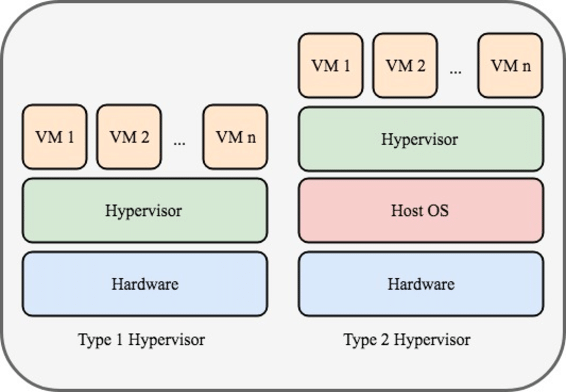
\includegraphics[scale=0.55]{gambar/Type-1-and-type-2-hypervisors.png}
  \caption{Hypervisor Tipe 1 dan Tipe 2 \parencite{nfv}}
  \label{fig:arsitektur-hypervisor-1-2}
\end{figure}

Hypervisor memiliki beberapa fitur untuk mengelola \emph{virtual machine}, yaitu:

\begin{enumerate}
  
  \item Abstraksi sumber daya fisik. Hypervisor menyediakan abstraksi untuk sumber
    daya dari mesin fisik. Abstraksi ini membatasi sumber daya fisik dari mesin yang
    nantinya bisa dipakai oleh \emph{virtual machine}. Dengan abstraksi ini,
    \emph{virtual machine} tidak perlu mengetahui sistem operasi dan \emph{hardware}
    dari \emph{host}.

  \item Isolasi sumber daya fisik. Hypervisor membagi sumber daya fisik dari \emph{host}
    dan membuat entitas terisolasi. Hypervisor memperbolehkan setiap \emph{virtual machine} 
    untuk berjalan secara independen. \emph{Virtual machine} yang terkompromisasi tidak
    akan mengganggu atau membuat \emph{virtual machine} lain juga terkompromisasi. Hal
    tersebut merupakan fungsi dari fitur isolasi sumber daya fisik. Tiap-tiap sumber daya fisik
    yang digunakan oleh \emph{virtual machine} saling terisolasi satu sama lain dan juga
    terisolasi dari sumber daya fisik yang digunakan oleh sistem operasi \emph{host}.

  \item Pengembalian kondisi \emph{virtual machine}. Setiap \emph{virtual machine} menggunakan
    sumber daya fisik dalam bentuk \emph{virtual disk}. \emph{Virtual disk} ini disimpan
    dalam bentuk \emph{file}. \emph{Virtual machine} menyimpan \emph{snapshot} dari \emph{virtual disk}
    dari waktu ke waktu atau setiap ada perubahan dalam \emph{virtual disk} tersebut. Ketika \emph{virtual machine}
    mengalami kendala atau masalah, \emph{virtual machine} dapat dikembalikan ke kondisi \emph{virtual disk}
    yang masih berfungsi sebelumnya.

\end{enumerate}

\subsubsection{QEMU}

QEMU \parencite{qemu-website} adalah emulator dan \emph{virtualizer} mesin generik dan bersifat sumber terbuka.
QEMU dapat digunakan dengan beberapa cara tetapi yang paling umum digunakan adalah sebagai
emulasi sistem. Hasil emulasi sistem tersebut menyediakan model virtual dari sebuah mesin
utuh seperti CPU, memori, dan emulasi perangkat untuk menjalankan sistem operasi \emph{guest}.
Pada mode tersebut, CPU bekerja secara teremulasi sepenuhnya atau dapat bekerja sama
dengan hypervisor seperti KVM, Xen, atau hypervisor lainnya untuk menjalankan sistem
operasi \emph{guest} secara langsung di CPU \emph{host}.
Dalam implementasi tugas akhir ini, QEMU akan digunakan sebagai emulator dan KVM
akan digunakan sebagai hypervisor. Penjelasan mengenai KVM akan dijelaskan pada bab \ref{sec:kvm}.

\subsubsection{KVM}
\label{sec:kvm}

KVM atau \emph{Kernel-based Virtual Machine} \parencite{kvm-website} merupakan \emph{full virtualizer} sumber terbuka
untuk Linux yang memiliki x86 \emph{hardware} dan salah satu hypervisor tipe 1. KVM memiliki ekstensi untuk dua jenis
CPU, yaitu Intel dengan teknologi Intel VT dan AMD dengan teknologi AMD-V. KVM terintegrasi
langsung dengan kernel Linux mulai versi 2.6.20 dengan menyediakan modul kernel kvm.ko yang dapat dimuat.
Modul tersebut menyediakan inti dari infrastruktur untuk virtualisasi. Selain itu, KVM
juga menyediakan modul spesifik untuk Intel yaitu kvm-intel.ko dan untuk AMD yaitu
kvm-amd.ko. Dengan menggunakan KVM, sistem operasi Linux dapat menjalankan satu atau lebih
mesin virtual. Setiap mesin virtual memiliki \emph{hardware} virtual pribadi seperti
\emph{network card}, \emph{disk}, dan \emph{graphics adapter}.

\subsection{Libvirt}
\label{sec:libvirt}

Libvirt adalah \emph{toolkit} sumber terbuka untuk mengelola platform virtualisasi.
Libvirt memudahkan proses pengelolaan platform virtualisasi dengan menyediakan API yang konsisten
dan terstandardisasi untuk banyak jenis hypervisor seperti KVM, QEMU, Xen, VMWare,
dan lain-lain. API tersebut disediakan oleh libvirt sebagai antarmuka interaksi dengan hypervisor.

Libvirt menggunakan arsitektur klien-server, dimana server dari Libvirt berupa daemon
bernama libvirtd yang akan berinteraksi dengan hypervisor yang digunakan dan klien akan
berkomunikasi dengan server atau libvirtd menggunakan protokol yang sudah ditetapkan.
Proses komunikasi antara klien dan server dapat dilakukan dengan beberapa cara, salah
satunya adalah secara terprogram dengan menggunakan bahasa pemrograman.

Libvirt menyediakan \emph{bindings} untuk beberapa bahasa pemrograman seperti Golang, C, Python, dan
lain-lain. Selain itu, Libvirt juga mendukung banyak fitur dari virtualisasi seperti
membuat \emph{virtual machine}, menghentikan \emph{virtual machine} dan menghapus \emph{virtual machine}.

\subsection{\emph{Network Bridge}}
\label{sec:network-bridge}

\emph{Network bridge} merupakan sebuah perangkat yang terdapat pada lapisan ke-dua atau \emph{data link layer} pada
model konseptual OSI atau \emph{Open System Interconnection}. OSI memecah komunikasi jaringan
menjadi tujuh bagian atau lapisan. Model OSI memudahkan berbagai sistem komunikasi
untuk berkomunikasi menggunakan protokol standar.

\emph{Network bridge} menggabungkan dua atau lebih segmen jaringan sehingga terlihat
seperti satu jaringan yang besar. Fungsi dari \emph{network bridge} adalah untuk meneruskan
trafik atau data berdasarkan alamat dari MAC (\emph{Media Access Control}). Tujuan
penggunaan \emph{network bridge} adalah memperluas jaringan lokal atau
membagi jaringan yang lebih besar untuk meningkatkan kinerja dan keamanan \parencite{network-bridge}.

\subsubsection{Linux \emph{Bridge}}

Linux \emph{bridge} adalah salah satu implementasi dari \emph{network bridge} dalam sistem
operasi Linux. Implementasi Linux \emph{bridge} pada kernel Linux sudah
terintegrasi sejak versi 2.4 \parencite{linux-foundation-bridge-website}.
Pada Linux \emph{bridge}, \emph{network bridge} diimplementasikan pada tingkat
perangkat lunak pada kernel Linux. Sama seperti kegunaan dari \emph{network bridge},
Linux \emph{bridge} dapat menyambungkan antarmuka jaringan satu dengan antarmuka jaringan
lainnya yang ada pada sebuah mesin Linux. Visualisasi dari Linux \emph{bridge}
dapat dilihat pada gambar \ref{fig:linux-bridge}

\begin{figure}[H]
  \centering
  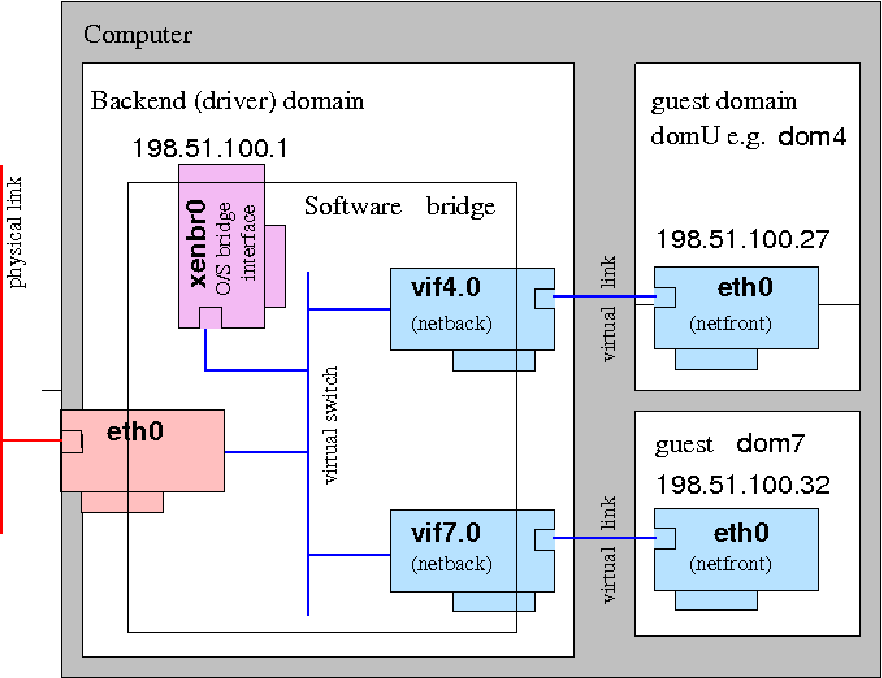
\includegraphics[scale=0.3]{gambar/linux-bridge.png}
  \caption{Visualisasi Linux \emph{Bridge} \parencite{Singh861571}}
  \label{fig:linux-bridge}
\end{figure}

Pada sistem operasi Linux, \emph{virtual machine} yang dibuat dapat mengutilisasi Linux
\emph{bridge} untuk tersambung dengan jaringan lokal yang sama dengan \emph{host}.
Dengan begitu, alamat IP yang didapat oleh \emph{virtual machine} berada dalam jangkauan
yang sama dengan jangkauan dari alamat IP \emph{host}, sehingga \emph{virtual machine} tersebut
terlihat sebagai satu mesin fisik tersendiri.

\subsection{RPC}

RPC atau \emph{Remote Procedure Call} adalah sebuah paradigma komunikasi antar program
melalui jaringan internet. RPC memungkinkan sebuah program untuk mengeksekusi sebuah
prosedur atau fungsi yang terdapat pada komputer lain seperti mengeksekusi prosedur
atau fungsi tersebut secara lokal. Konsep mengenai RPC pertama kali dikenalkan oleh
Bruce Jay Nelson melalui disertasinya yang berjudul "Remote Procedure Call" \parencite{rpc}.

Gambaran komunikasi melalui RPC dapat dilihat pada gambar \ref{fig:rpc-communication}.
Pada gambar tersebut, mesin C memanggil prosedur yang terdapat pada mesin S melalui
hubungan internet. Setelah itu, mesin S mengembalikan hasil dari prosedur tersebut
ke mesin C. Hasil prosedur dari mesin S tersebut dapat digunakan oleh
mesin C untuk menjalankan tugasnya tanpa perlu menjalankan prosedur tersebut
secara lokal di mesin C.

\begin{figure}[H]
  \centering
  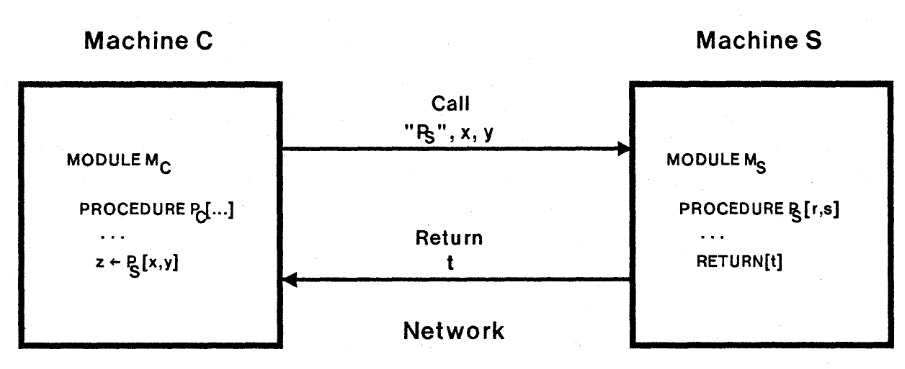
\includegraphics[scale=0.3]{gambar/rpc-communication.png}
  \caption{Komunikasi RPC \parencite{rpc}}
  \label{fig:rpc-communication}
\end{figure}

Gambaran lainnya dari proses RPC terdapat pada gambar \ref{fig:rpc-communication-2}.
Pada gambar tersebut, mesin yang memanggil prosedur atau fungsi melalui RPC memiliki sebuah
\emph{stub} atau \emph{template} dari prosedur atau fungsi yang ingin dipanggil. Mesin
tempat prosedur dipanggil juga memiliki \emph{stub} dari fungsi atau prosedur tersebut namun
mesin tersebut menyediakan \emph{logic} dalam menjalankan fungsi atau prosedur. \emph{Stub}
pada mesin yang memanggil merupakan \emph{identifier} dari fungsi atau prosedur apa yang ingin
dipanggil di mesin tempat fungsi atau prosedur dijalankan.

\begin{figure}[H]
  \centering
  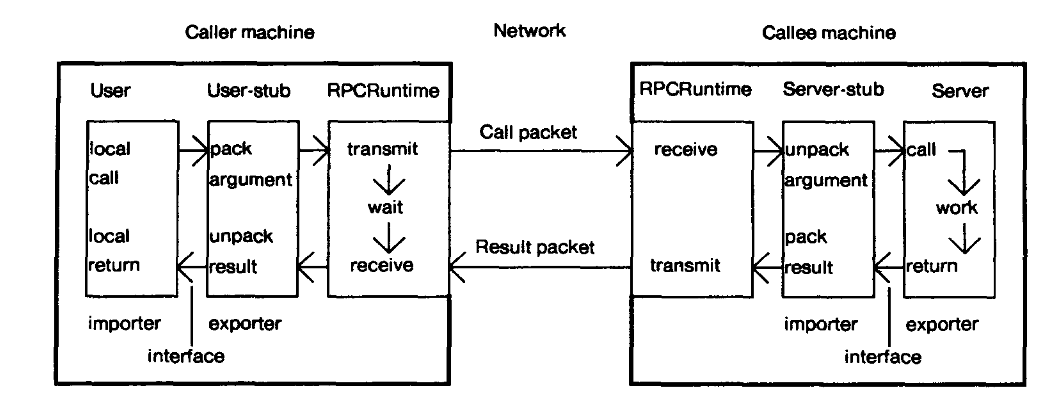
\includegraphics[scale=0.35]{gambar/rpc-communication-2.png}
  \caption{Komunikasi RPC \parencite{implementing-rpc}}
  \label{fig:rpc-communication-2}
\end{figure}

\subsubsection{gRPC}

gRPC adalah implementasi dari RPC yang diciptakan oleh Google. Sama seperti sistem
yang mengimplementasikan sistem RPC, gRPC menggunakan konsep mendefinisikan sebuah \emph{service},
menentukan metode yang bisa dipanggil dari jarak jauh beserta parameter dan tipe data yang
dikembalikan oleh metode tersebut. Secara \emph{default}, gRPC menggunakan protocol buffers
sebagai \emph{Interface Definition Language} (IDL) untuk mendefinisikan antarmuka \emph{service}
dan struktur dari \emph{payload} yang diperlukan oleh \emph{service}. Gambaran garis besar
komunikasi gRPC terdapat pada gambar \ref{fig:grpc-top-level}.

\begin{figure}[H]
  \centering
  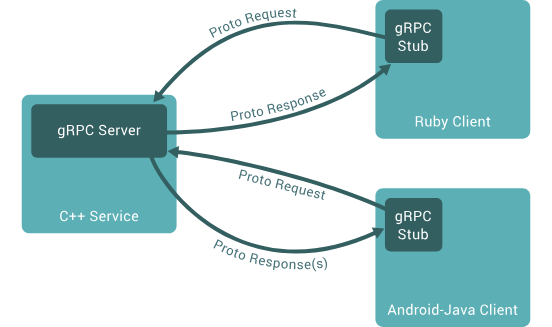
\includegraphics[scale=0.5]{gambar/grpc-usage-image.png}
  \caption{Komunikasi gRPC \parencite{grpc-website-docs-overview}}
  \label{fig:grpc-top-level}
\end{figure}

\subsection{Cloud-init}

Cloud-init merupakan sebuah program sumber terbuka yang berjalan pada saat
\emph{booting} awal dari sebuah \emph{virtual machine} atau \emph{cloud instance}.
Fungsi utama dari Cloud-init adalah untuk menyesuaikan \emph{virtual machine}
atau \emph{cloud instance} dengan data yang diberikan oleh pengguna. Dengan begitu,
setiap \emph{virtual machine} atau \emph{cloud instance} yang dijalankan dengan Cloud-init
akan identik dengan semua konfigurasi yang digunakan. Fungsi tersebut mempermudah dalam 
mengotomisasi konfigurasi awal dari \emph{virtual machine} atau \emph{cloud instance}.

Cloud-init mendukung banyak jenis konfigurasi. Beberapa jenis konfigurasi yang dapat digunakan
pada Cloud-init adalah sebagai berikut:

\begin{enumerate}
  
  \item Antarmuka Jaringan

    Cloud-init dapat mengatur antarmuka jaringan yang digunakan pada \emph{virtual machine}
    atau \emph{cloud instance}. Selain itu, Cloud-init juga dapat menyesuaikan konfigurasi
    antarmuka jaringan tersebut seperti jenis IP, alamat IP, dan lain-lain

  \item \emph{User} dan \emph{Group} Linux

    Selain mengkonfigurasi jaringan, Cloud-init juga mendukung pembuatan \emph{user} dan \emph{group} pada
    sistem operasi Linux pada saat pertama kali \emph{booting}. Konfigurasi lain seperti nama \emph{user},
    nama \emph{group}, \emph{group} dari \emph{user}, dan \emph{password} dari \emph{user} juga didukung
    oleh Cloud-init.

  \item Instalasi \emph{package} dengan \emph{package manager}

    Cloud-init mendukung instalasi \emph{package} menggunakan \emph{package manager} dari distribusi Linux
    seperti Ubuntu. 

  \item \emph{Shell Scripts}

    Cloud-init mendukung penggunaan \emph{shell script} pada saat proses Cloud-init
    berjalan. \emph{Shell scripts} dapat digunakan untuk konfigurasi yang tidak didukung
    oleh Cloud-init seperti menjalankan aplikasi \emph{command line interface} untuk mengunduh
    menggunakan wget dan lain-lain.

\end{enumerate}

\subsection{Golang}

Golang merupakan bahasa pemrograman yang diciptakan oleh Google dan pada 
tahun 2009 dibagi secara publik. \emph{Libraries}
serta fitur-fitur yang ditawarkan oleh Golang seperti \emph{pointer} dan \emph{error as a value}
dapat digunakan dalam banyak kebutuhan seperti pembuatan \emph{services}, \emph{command line interface},
dan lain-lain \parencite{go-website}.
